% Created 2021-01-13 Wed 13:14
% Intended LaTeX compiler: pdflatex
\documentclass[presentation]{beamer}
\usepackage[utf8]{inputenc}
\usepackage[T1]{fontenc}
\usepackage{graphicx}
\usepackage{grffile}
\usepackage{longtable}
\usepackage{wrapfig}
\usepackage{rotating}
\usepackage[normalem]{ulem}
\usepackage{amsmath}
\usepackage{textcomp}
\usepackage{amssymb}
\usepackage{capt-of}
\usepackage{hyperref}
\usetheme{UoB}
\author{Mark Blyth}
\date{}
\title{Multi-timescale systems and slow-fast analysis}
\hypersetup{
 pdfauthor={Mark Blyth},
 pdftitle={Multi-timescale systems and slow-fast analysis},
 pdfkeywords={},
 pdfsubject={},
 pdfcreator={Emacs 27.1 (Org mode 9.3)}, 
 pdflang={English}}
\begin{document}

\maketitle

\section{1 Intro}
\label{sec:org66a5869}
\begin{frame}[label={sec:org14d0dda}]{Why multiple timescales?}
Biological systems consist of interacting parts operating over many timescales
\vfill
\begin{itemize}
\item Accurate models need a combination of slowly and rapidly changing variables
\item Doing anything useful with these models requires ways of understanding timescale interactions
\end{itemize}
\vfill
Simplest example
\[\dot{x} = f(x,y)\]
\[\dot{y} = \varepsilon g(x,y)\]
\end{frame}

\begin{frame}[label={sec:orgfaa04fa}]{Subsystems and timescale separations}
\begin{itemize}
\item Consider \(\varepsilon\to0\)
\item Let \(\tau = \varepsilon t\)
\end{itemize}
\vfill

\begin{columns}
\begin{column}{0.5\columnwidth}
Fast subsystem:
\begin{align}
\frac{\mathrm{d}x}{\mathrm{d}t} &= f(x,y) \\ \nonumber
\frac{\mathrm{d}y}{\mathrm{d}t} &= 0
\end{align}
\end{column}

\begin{column}{0.5\columnwidth}
Slow subsystem:
\begin{align}
f(x,y) &= 0 \\ \nonumber
\frac{\mathrm{d}y}{\mathrm{d}\tau} &= g(x,y)
\end{align}
\end{column}
\end{columns}
\end{frame}

\begin{frame}[label={sec:orgedf5ed7}]{Example systems}
Mathematically interesting, and biologically useful: we can express lots of biology like this
\vfill
\begin{itemize}
\item Pulsing behaviours
\begin{itemize}
\item Heart beats, neuron spikes, hormone pulses
\end{itemize}
\end{itemize}
\vfill
\begin{itemize}
\item Mixed-mode oscillations
\begin{itemize}
\item Chemical systems, neuron voltage dynamics, pituitary cells
\end{itemize}
\end{itemize}
\vfill
\begin{itemize}
\item Can classify neurons based on their fast subsystem topology
\end{itemize}
\end{frame}

\section{2 Relaxation oscillations and canards}
\label{sec:org064e600}
\begin{frame}[label={sec:org58ee1bd},plain]{A test model}
van-der-Pol oscillator is the classic planar slow-fast system; we consider a topologically equivalent bio model

\begin{align}
\frac{\mathrm{d}V}{\mathrm{d}t} &= -(I_{Ca} + I_{Kdr} + I_{KATP} + I_{Ks} + I_l) \\ \nonumber
\frac{\mathrm{d}s}{\mathrm{d}t} &= \frac{s_\infty(V) - s}{\tau_s}
\end{align}

\begin{center}
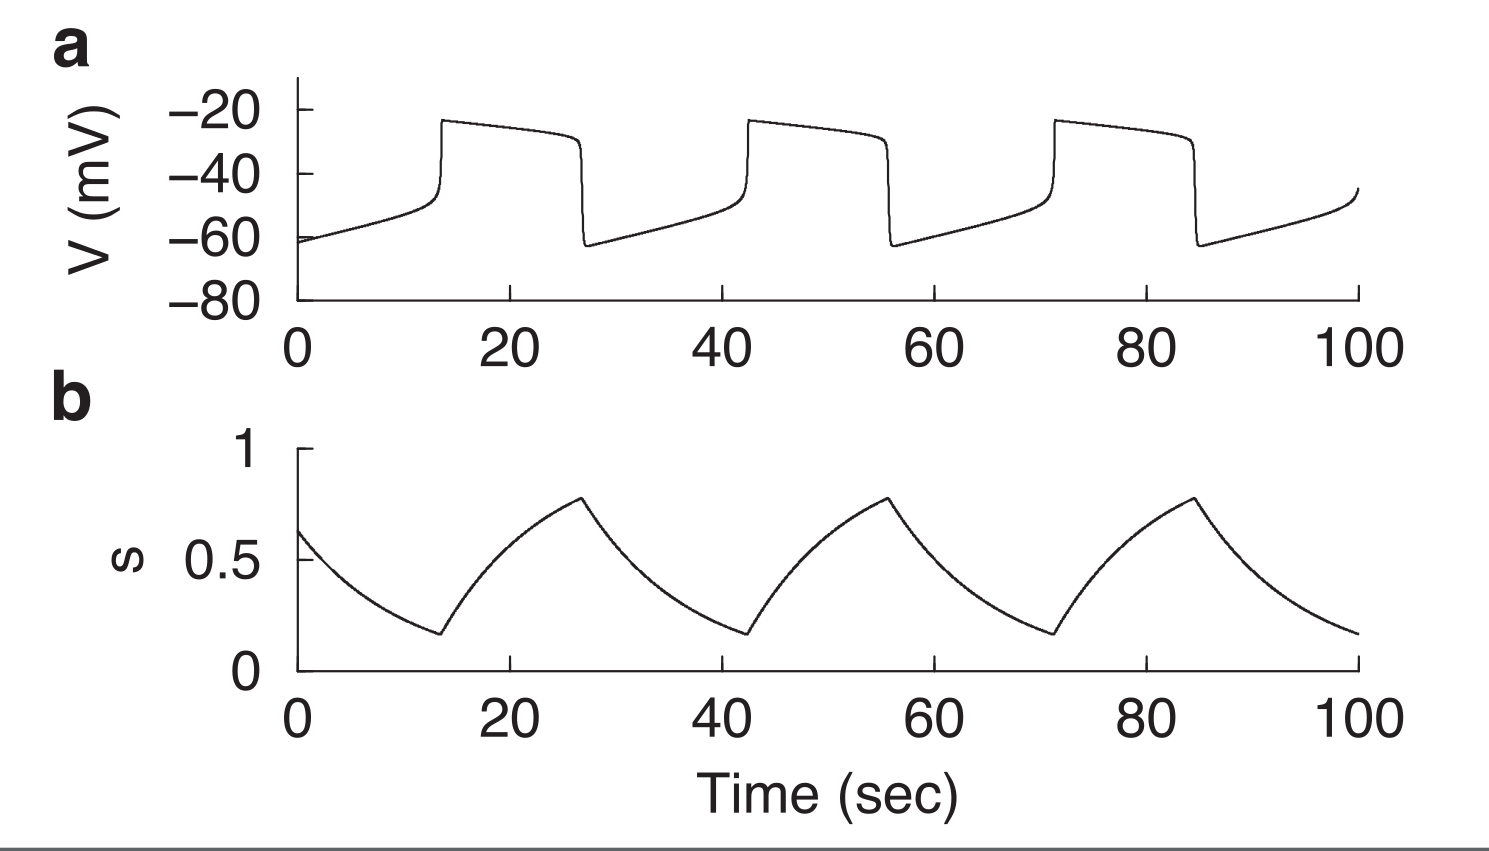
\includegraphics[width=.7\textwidth]{./dynamics.png}
\end{center}
\end{frame}

\begin{frame}[label={sec:orgca6256b}]{Planar dynamics}
Behaviours shown are typical of slow-fast systems
\begin{itemize}
\item States settle to equilibrium of fast subsystem
\item Equilibrium evolves, disappears, reappears through changes in slow subsystem
\end{itemize}

\begin{center}
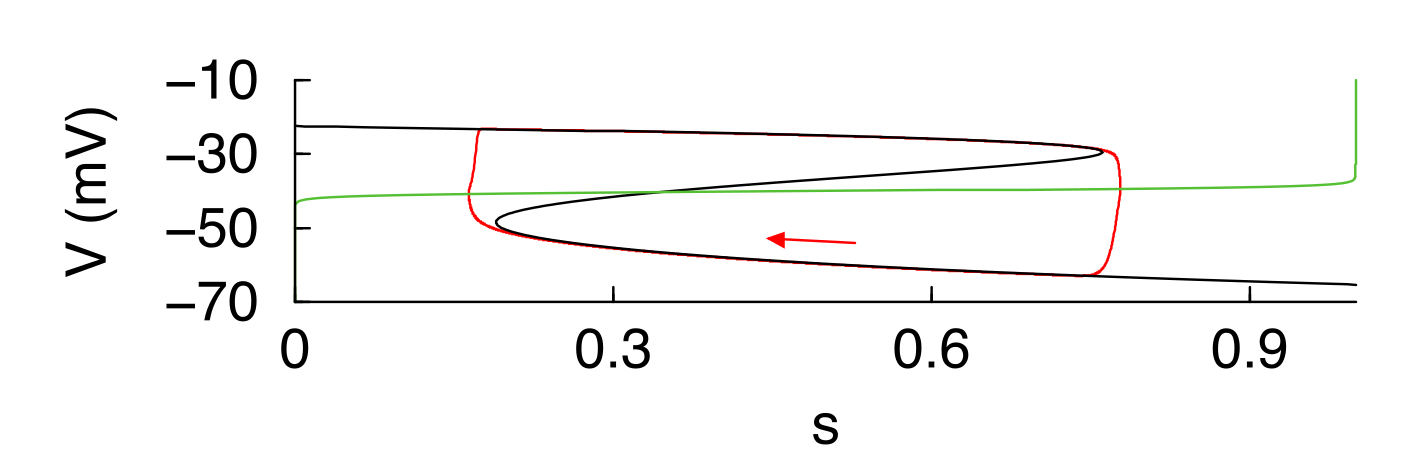
\includegraphics[width=.9\linewidth]{./phaseplane.png}
\end{center}
\end{frame}

\section{3 Bursting}
\label{sec:org42980c5}
\begin{frame}[label={sec:org224f664}]{Higher dimensions}
\begin{itemize}
\item Higher-dimensional models can also show relaxation oscillations, plus more
\item Unlike the planar case, the fast subsystem attractor might no longer satisfy \(f(x,y)=0\)
\end{itemize}
\vfill
Consider our neuron model again, without the steadystate assumption on \(I_{Kdr}\)

\begin{align}
\frac{\mathrm{d}V}{\mathrm{d}t} &= -(I_{Ca} + I_{Kdr} + I_{KATP} + I_{Ks} + I_l) \\ \nonumber
\frac{\mathrm{d}s}{\mathrm{d}t} &= \frac{s_\infty(V) - s}{\tau_s} \\
\frac{\mathrm{d}n}{\mathrm{d}t} &= \frac{n_\infty(V) - n}{\tau_n} \nonumber
\end{align}
\end{frame}

\begin{frame}[label={sec:org76d7187},plain]{Bursting}
Our new model produces bursting oscillations!

\begin{center}
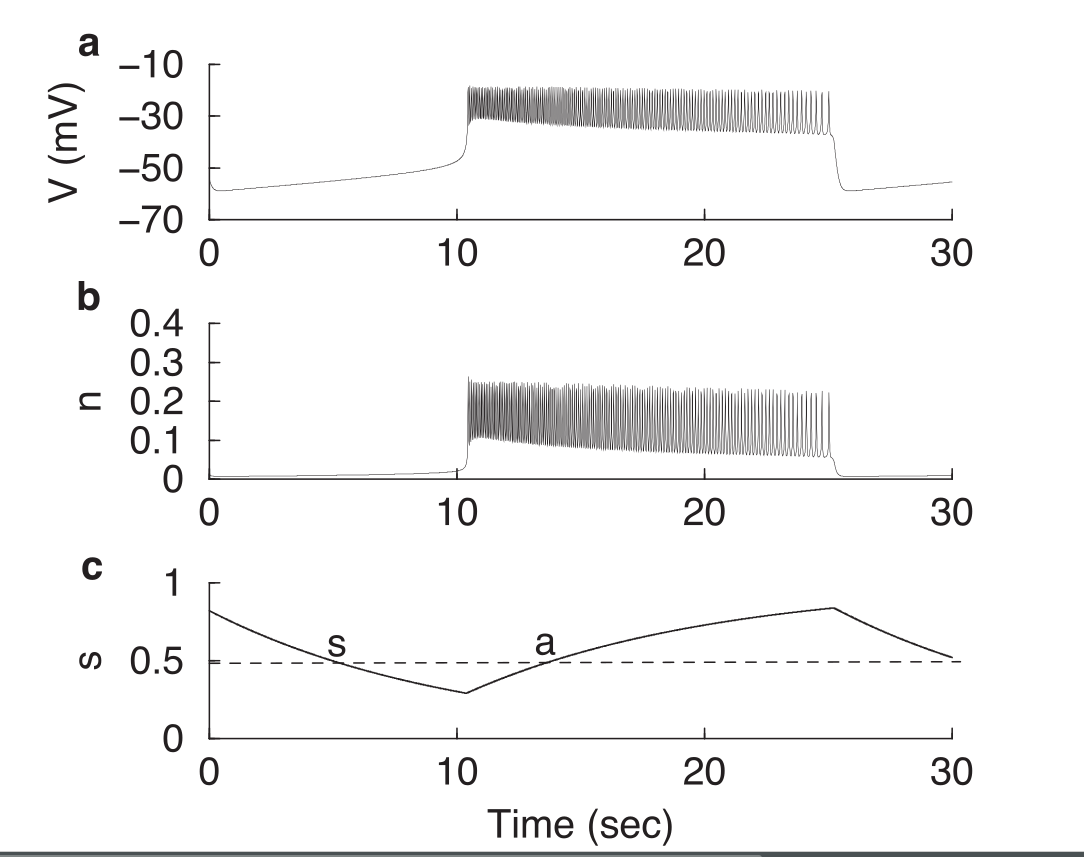
\includegraphics[width=.8\textwidth]{./burst.png}
\end{center}
\end{frame}

\begin{frame}[label={sec:org8ff57eb},plain]{Busting phase plane}
\begin{center}
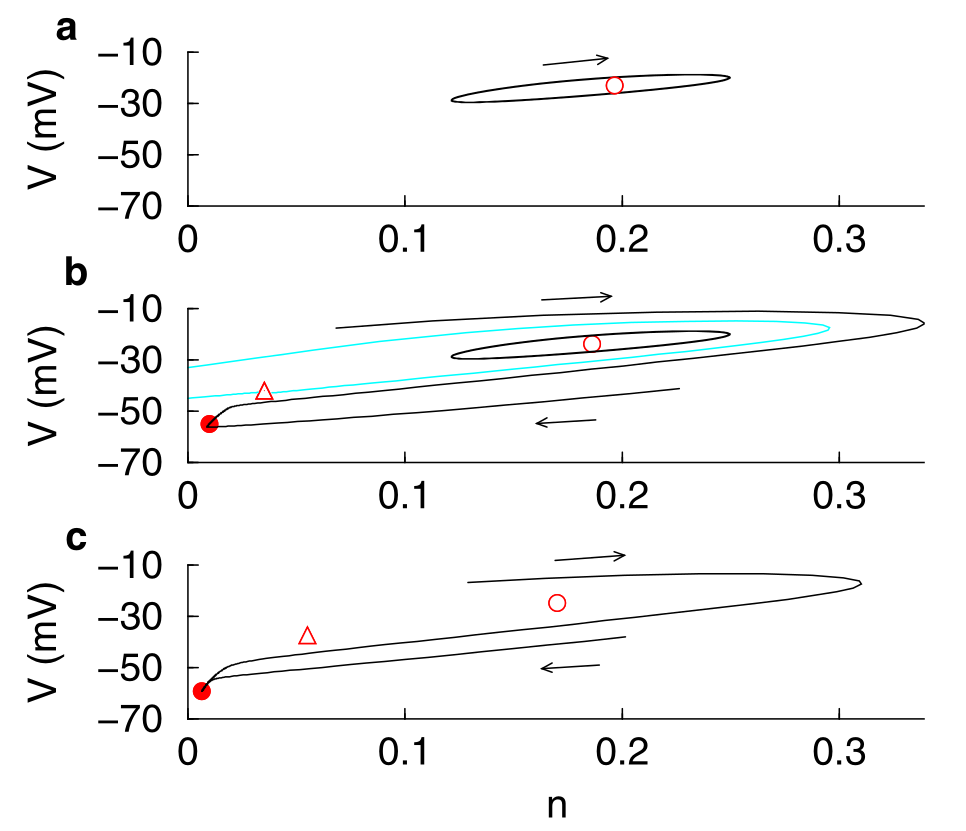
\includegraphics[width=.8\textwidth]{./burstplane.png}
\end{center}
\end{frame}

\begin{frame}[label={sec:org3cc1abf}]{Higher dimensional models}
What happens if we have two slow variables?

\begin{align}
\frac{\mathrm{d}V}{\mathrm{d}t} &= -(I_{Ca} + I_{Kdr} + I_{Ks1} + I_{Ks2} + I_l) \\ \nonumber
\frac{\mathrm{d}n}{\mathrm{d}t} &= \frac{n_\infty(V) - n}{\tau_n} \\ \nonumber
\frac{\mathrm{d}s_1}{\mathrm{d}t} &= \frac{s_{1\infty}(V) - s_1}{\tau_{s1}} \\ \nonumber
\frac{\mathrm{d}s_2}{\mathrm{d}t} &= \frac{s_{2\infty}(V) - s_2}{\tau_{s2}} \nonumber
\end{align}

Same model as earlier, only we now have two fast variables \(V\) and \(n\), slow variable \(s_1\), and super-slow variable \(s_2\)
\end{frame}

\begin{frame}[label={sec:org3bad4d3},plain]{Higher dimensional models}
\begin{itemize}
\item Previously, the slow variable switched spiking on and off
\item Now, the very-slow variable switches the system from bursting to either quiescence or tonic spiking
\item The slow-variable oscillates, and changes direction during the active phase
\end{itemize}


\begin{center}
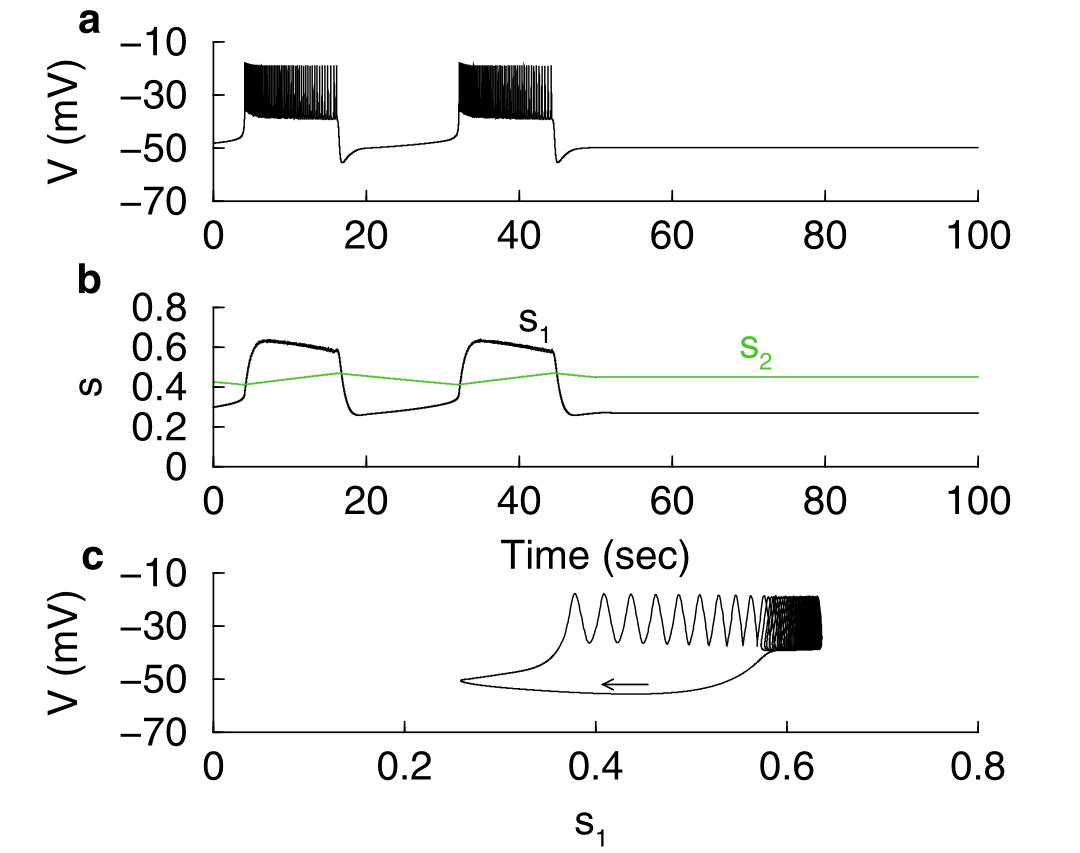
\includegraphics[width=.74\textwidth]{./phantomts.png}
\end{center}
\end{frame}

\begin{frame}[label={sec:org1b23cbe}]{More dimensions = more robustness}
Planar bursting requires
\begin{itemize}
\item Bistability in the fast subsystem
\item The slow-subsystem nullcline to intersect in the right place
\end{itemize}
\vfill
This limits the region of parameter space in which bursting can occur
\begin{itemize}
\item Not very good -- biology is noisy and imprecise; if we need very specific values, things probably won't work
\item Adding additional slow dynamics makes things more robuts
\item Interpretation: instead of shifting the state around, the slow variables shift the entire bifurcation diagram back and forth
\end{itemize}
\end{frame}
\section{4 Robust non-planar canards}
\label{sec:org69bcf66}
\begin{frame}[label={sec:orge673fd0}]{Canards}
\begin{itemize}
\item Canards cause a rapid transition from quiescence to spiking
\item Solution follows fast-subsystem unstable manifold
\begin{itemize}
\item Torus canards follow branches of UPO
\end{itemize}
\item Canards are non-robust in planar systems
\begin{itemize}
\item Appear in exponentially small region of parameter space
\end{itemize}
\item Complicated maths shows that these canards can appear robustly in non-planar systems
\end{itemize}

\begin{center}
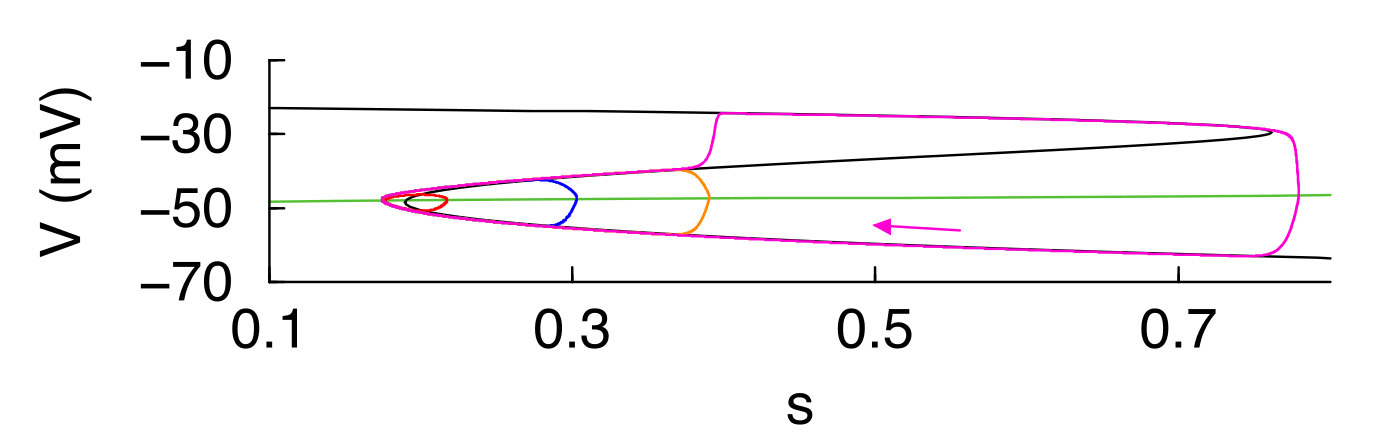
\includegraphics[width=.85\textwidth]{./planarcanard.png}
\end{center}
\end{frame}


\begin{frame}[label={sec:org6b8ee13},plain]{Mixed-mode oscillations}
\begin{itemize}
\item Canards arise from the existence of a folded node singularity
\item The same structure allows mixed-mode oscillations
\begin{itemize}
\item System oscillates between bigger and smaller oscillations
\end{itemize}
\end{itemize}

\begin{center}
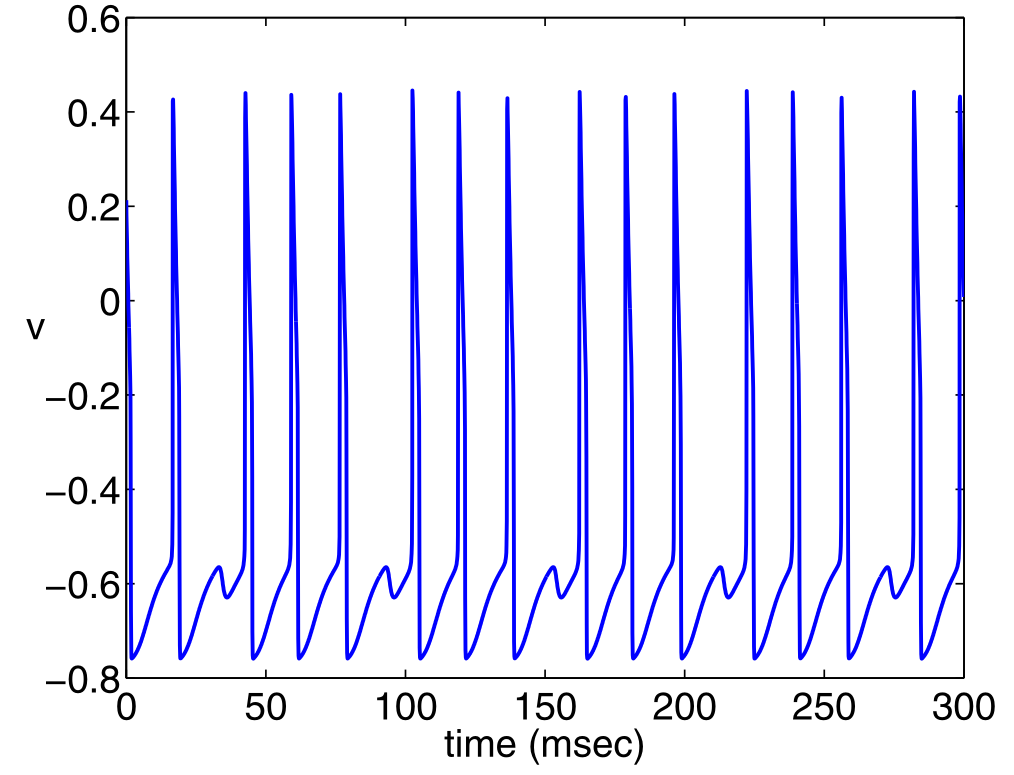
\includegraphics[width=.7\textwidth]{./mmo.png}
\end{center}
\end{frame}


\section{Why are biologists interested in these dynamics?}
\label{sec:orgd7198fe}
\begin{frame}[label={sec:org62c840d}]{Why are biologists interested?}
An example: the spinal cord
\vfill
\begin{itemize}
\item Synaptic coupling is all excitory
\begin{itemize}
\item Expectation: active network, due to positive feedbacks
\item Reality: mostly silent, occasional activity; \emph{why?}
\end{itemize}
\item Proposed model: synaptic depression; cells that fire together unwire
\begin{itemize}
\item Model shows relaxation oscillations
\end{itemize}
\item Predictions from multiscale analysis:
\begin{itemize}
\item Electrical perturbations will cause shift between activity and quiescence
\item Length of active, quiescent phase depends on perturbation timings
\end{itemize}
\item Predictions confirmed experimentally, elucidating spinal cord neurology
\end{itemize}
\end{frame}


\begin{frame}[label={sec:org912fc82}]{Practical issues}
\begin{itemize}
\item How do we identify how many timescales are present?
\item How do we identify what those timescales are?
\item How do we determine whether those timescales are distinct?
\item How do we best partition multiple timescales, when it's not obvious what should be fast, medium, or slow?
\end{itemize}
\end{frame}
\end{document}
